\part{The Riemann Hypothesis for Generalized Petersen Graphs}
\label{part:rh}

\section{The graph Riemann Hypothesis}\label{sec:grh}

Attached to a finite connected graph $X$ is its \emph{Ihara zeta function},
\[
  \zeta_X(u)=\prod_{[C]}\bigl(1-u^{\,\ell(C)}\bigr)^{-1},
\]
the product running over equivalence classes of primitive backtrackless
tailless closed paths, $\ell(C)$ the length. It is a graph-theoretic analogue
of the Riemann zeta function: it has an Euler product, a meromorphic
continuation, a functional equation, and a prime number theorem counting closed
geodesics. For a $(q+1)$-regular graph the substitution $u=q^{-s}$ makes the
analogy exact, and one may ask the corresponding question.

\begin{definition}[Riemann Hypothesis for a graph]
A $(q+1)$-regular graph $X$ satisfies the Riemann Hypothesis if
$\zeta_X(q^{-s})$ has no poles with $0<\mathrm{Re}\,s<1$ other than on the line
$\mathrm{Re}\,s=\tfrac12$.
\end{definition}

The point of the definition is the following equivalence, which converts an
analytic statement about a zeta function into a finite spectral one. It is
classical, following from the Ihara determinant formula; we take the statement
from Terras~\cite[Exercise 9]{terras}, where it appears in exactly this form.

\begin{theorem}[Ihara determinant formula; see \cite{terras}]\label{thm:grh}
A connected $(q+1)$-regular graph $X$ satisfies the Riemann Hypothesis if and
only if $X$ is \emph{Ramanujan}: every eigenvalue $\lambda$ of the adjacency
matrix with $|\lambda|\ne q+1$ satisfies $|\lambda|\le 2\sqrt q$.
\end{theorem}

The term is due to Lubotzky, Phillips and Sarnak~\cite{lps}, and the bound is
the best possible: $2\sqrt q$ is the spectral radius of the adjacency operator
on the universal covering tree, so a Ramanujan graph is one whose nontrivial
spectrum is as small as an infinite family can have it. Ramanujan graphs are
optimal expanders, which is why they matter outside spectral graph theory --
for communication networks, error-correcting codes, and derandomization.

Our graphs are cubic, $q+1=3$, so the threshold is
\[
  2\sqrt2 = 2.8284271247\ldots,
\]
and the trivial eigenvalues are $3$, always, and $-3$, exactly when the graph is
bipartite. We ask which generalized Petersen graphs are on the right side of it.

\begin{question}\label{q:main}
For which $n$ and $k$ does $P(n,k)$ satisfy the Riemann Hypothesis?
\end{question}

This is a natural question of a recognised kind. The analogue has been settled
for other families: Droll classified the Ramanujan unitary Cayley graphs, and
Le and Sander~\cite{lesander} classified the Ramanujan integral circulant
graphs of prime power order, in both cases finding that only finitely many
members qualify. For generalized Petersen graphs the spectrum has been
completely known since Gera and St\u{a}nic\u{a}~\cite{gs}, but we have not found
Question~\ref{q:main} raised anywhere: \cite{gs} itself contains no occurrence
of the words \emph{Ramanujan}, \emph{expander} or \emph{spectral gap}.

We answer it completely, for every $n$ and every $k$, in exact arithmetic. The
answer has four parts: a criterion reducing the question to the sign of one
integer polynomial; a change of variable after which the criterion is one fixed
region not depending on $k$; a Diophantine argument bounding $n$ uniformly in
$k$, so that the family is finite in both variables; and an exhaustive
certification of the finitely many survivors.

\section{The spectrum, and a criterion with no radicals}\label{sec:crit}

$P(n,k)$ is the cyclic cover of the two-vertex base of \S\ref{sec:covers} --
the same object this paper studies throughout -- and the block decomposition
used there is, on the zeta side, precisely the factorization of $\zeta_{P(n,k)}$
into Artin--Ihara $L$-functions over the characters of $\mathbb Z_n$. The
spectral form we need is the following, which is Theorem 2.4 of~\cite{gs}.

\begin{lemma}\label{lem:blocks}
The adjacency matrix of $P(n,k)$ is unitarily equivalent to
$\bigoplus_{j=0}^{n-1}M_j$, where
\[
  M_j=\begin{pmatrix}\alpha_j&1\\1&\beta_j\end{pmatrix},\qquad
  \alpha_j=2\cos\tfrac{2\pi j}{n},\qquad
  \beta_j=2\cos\tfrac{2\pi jk}{n}=2T_k(\alpha_j/2),
\]
with $T_k$ the Chebyshev polynomial of the first kind.
\end{lemma}

\begin{proof}
The rotation $\rho:i\mapsto i+1$ acts on $P(n,k)$ with the adjacency matrix in
its commutant, so the matrix decomposes over the characters
$\chi_j(a)=\zeta_n^{ja}$ of $\mathbb Z_n$. On the $\chi_j$ isotypic component
the outer cycle contributes $\zeta_n^{j}+\zeta_n^{-j}=\alpha_j$, the inner
$k$-step cycle contributes $\zeta_n^{jk}+\zeta_n^{-jk}=\beta_j$, and the spoke
contributes $1$ off the diagonal. The identity
$2\cos k\theta=2T_k(\cos\theta)$ gives the stated form of $\beta_j$.
\end{proof}

Deciding Question~\ref{q:main} directly from Lemma~\ref{lem:blocks} means
comparing $\bigl(\alpha+\beta\pm\sqrt{(\alpha-\beta)^2+4}\bigr)/2$ against
$2\sqrt2$ -- two nested irrationalities, and the comparison is decided at a band
edge where floating point is worth nothing. Both radicals can be cleared at
once, and what remains is a single polynomial with integer coefficients.

\begin{theorem}[Criterion]\label{thm:crit}
For $k\ge1$ define
\[
  D_k(u)=\bigl(7+4u\,T_k(u)\bigr)^2-8\bigl(2u+2T_k(u)\bigr)^2\ \in\ \mathbb Z[u],
  \qquad \deg D_k=2k+2 .
\]
Then both eigenvalues of $M_j$ lie in $[-2\sqrt2,2\sqrt2]$ if and only if
$D_k(u_j)\ge0$, where $u_j=\cos\frac{2\pi j}{n}$. The polynomial has degree
$2k+2$ and leading coefficient $4^{\,k+1}$.
\end{theorem}

\begin{proof}
Write $\alpha=\alpha_j$, $\beta=\beta_j$, $A=\alpha+\beta$, $P=\alpha\beta$.
The characteristic polynomial of $M_j$ is $\lambda^2-A\lambda+(P-1)$, with roots
$\lambda_\pm=\bigl(A\pm\sqrt{(\alpha-\beta)^2+4}\bigr)/2$.

For the upper constraint, $\lambda_+\le2\sqrt2$ is
$\sqrt{(\alpha-\beta)^2+4}\le4\sqrt2-A$. Since $|\alpha|,|\beta|\le2$ we have
$|A|\le4<4\sqrt2$, so the right-hand side is positive and squaring is an
equivalence, not merely an implication:
\[
  (\alpha-\beta)^2+4\ \le\ 32-8\sqrt2\,A+A^2 .
\]
Because $A^2-(\alpha-\beta)^2=4P$, this simplifies to $4\le32-8\sqrt2A+4P$,
that is $2\sqrt2\,A-P\le7$. Symmetrically $\lambda_-\ge-2\sqrt2$ is equivalent
to $-2\sqrt2\,A-P\le7$. The two together say
\[
  2\sqrt2\,|A|\ \le\ 7+P .
\]
Now $|P|=|\alpha\beta|\le4$, so $7+P\ge3>0$: the right-hand side is again
positive, so squaring is again an equivalence, giving $8A^2\le(7+P)^2$. Finally
$\alpha=2u$ and $\beta=2T_k(u)$, so $A=2u+2T_k(u)$ and $P=4u\,T_k(u)$, and
$(7+P)^2-8A^2=D_k(u)$.

For the degree: $T_k$ has degree $k$ and leading coefficient $2^{k-1}$, so
$\bigl(7+4uT_k\bigr)^2$ has degree $2k+2$ with leading coefficient
$\bigl(4\cdot2^{k-1}\bigr)^2=4^{\,k+1}$, while $8\bigl(2u+2T_k\bigr)^2$ has
degree only $2k$. Nothing cancels, so $\deg D_k=2k+2$ with leading coefficient
$4^{\,k+1}$.
\end{proof}

\begin{corollary}[Ramanujan, polynomially]\label{cor:crit}
$P(n,k)$ satisfies the Riemann Hypothesis if and only if
\[
  D_k\!\left(\cos\tfrac{2\pi j}{n}\right)\ \ge\ 0
  \qquad\text{for every }j\in\{1,\dots,n-1\}\text{ with }2j\ne n\text{ or }k
  \text{ even.}
\]
\end{corollary}

\begin{proof}
$P(n,k)$ is connected -- the outer cycle is connected and every inner vertex
carries a spoke -- and cubic, so by Theorem~\ref{thm:grh} the question is
whether every eigenvalue of modulus $\ne3$ has modulus $\le2\sqrt2$. By
Lemma~\ref{lem:blocks} the spectrum is $\bigcup_j\mathrm{spec}(M_j)$.

The block $M_0$ has $\alpha=\beta=2$, hence eigenvalues $3$ and $1$. If $n$ is
even and $k$ odd then $P(n,k)$ is bipartite and $M_{n/2}$ has
$\alpha=\beta=-2$, hence eigenvalues $-1$ and $-3$. No other block has $\pm3$
as an eigenvalue, since $3$ and $-3$ have multiplicity one in a connected
$3$-regular graph (and $-3$ occurs only in the bipartite case). So the two
excluded indices contribute the trivial eigenvalues together with $1$ and $-1$
respectively, both of modulus $1\le2\sqrt2$; every other index contributes only
nontrivial eigenvalues. Apply Theorem~\ref{thm:crit} at each of those.
\end{proof}

The reduction is worth pausing on. The side condition $7+P\ge0$ that licensed
the second squaring is \emph{never} binding, since $|4u\,T_k(u)|\le4$ on
$[-1,1]$ forces $7+4uT_k(u)\ge3$. So the entire Riemann Hypothesis for
$P(n,k)$ -- an analytic statement about the poles of a zeta function -- has
become the assertion that one integer polynomial is nonnegative at $n-1$
cyclotomic points. That is a statement our exact machinery can certify
outright, and \S\ref{sec:ramcert} does.

\section{The criterion without \texorpdfstring{$k$}{k}}\label{sec:corner}

Theorem~\ref{thm:crit} gives one polynomial per $k$, of degree growing with
$k$. There is a change of variable after which $k$ leaves the geometry
entirely, and what is left is a single fixed region that does not depend on
$k$ at all.

\begin{theorem}[Corner criterion]\label{thm:corner}
Put
\[
  x=\cos\frac{\pi j(k+1)}{n},\qquad
  y=\cos\frac{\pi j(k-1)}{n},\qquad
  Q(x,y)=4x^{2}+4y^{2}-8\sqrt2\,|xy|+3 .
\]
Both eigenvalues of $M_j$ lie in $[-2\sqrt2,2\sqrt2]$ if and only if
$Q(x,y)\ge0$. Hence $P(n,k)$ satisfies the Riemann Hypothesis if and only if
$Q(x,y)\ge0$ at every nontrivial index. The form $Q$ does not involve $k$.
\end{theorem}

\begin{proof}
$D_k=(7+P)^{2}-8A^{2}$ is a difference of squares, so over $\mathbb Q(\sqrt2)$
it factors as $D_k=f_-f_+$ with
\[
  f_\pm=7+P\pm2\sqrt2\,A ,
\]
each of degree $k+1$ in $u$. These factors are not new objects: the proof of
Theorem~\ref{thm:crit} produced exactly them, $f_-\ge0$ being
$\lambda_+\le2\sqrt2$ and $f_+\ge0$ being $\lambda_-\ge-2\sqrt2$. What is
required is that \emph{both} be nonnegative. They cannot both be negative,
since
\[
  f_-+f_+=2(7+P)\ge6>0
\]
by $|P|\le4$; so the product is nonnegative exactly when both factors are,
which is why the single inequality $D_k\ge0$ was equivalent to the pair.

Now set $t=2\pi j/n$, so $u=\cos t$ and $x=\cos\frac{(k+1)t}{2}$,
$y=\cos\frac{(k-1)t}{2}$. From $2\cos t\cos kt=\cos(k+1)t+\cos(k-1)t$ and
$\cos(k\pm1)t=2\cos^{2}\frac{(k\pm1)t}{2}-1$,
\[
  P=4\cos t\cos kt=2\bigl((2x^{2}-1)+(2y^{2}-1)\bigr)=4x^{2}+4y^{2}-4 ,
\]
and from $\cos t+\cos kt=2\cos\frac{(k+1)t}{2}\cos\frac{(k-1)t}{2}$,
\[
  A=2(\cos t+\cos kt)=4xy .
\]
Hence $7+P=3+4x^{2}+4y^{2}$ and
\[
  f_\mp=3+4x^{2}+4y^{2}\mp8\sqrt2\,xy ,
\]
whose minimum over the two signs is $4x^{2}+4y^{2}-8\sqrt2\,|xy|+3=Q(x,y)$.
Both are nonnegative exactly when $Q\ge0$.
\end{proof}

The content of the theorem is that $k$ has moved out of the region and into the
map. For every $k$ the question is asked about the same subset of the square.

\begin{corollary}[The forbidden set]\label{cor:lens}
\[
  Q=4\bigl(|x|-(\sqrt2+1)|y|\bigr)\bigl(|x|-(\sqrt2-1)|y|\bigr)+3 ,
\]
so $\{Q<0\}$ is bounded by a hyperbola with asymptotes
$|x|=(\sqrt2\pm1)|y|$. Its intersection with the square $[-1,1]^{2}$ is four
congruent regions, one at each corner $(\pm1,\pm1)$, each meeting the two
sides through its corner in segments of length exactly $\tfrac32-\sqrt2$ and
having area
\[
  \tfrac32-\sqrt2+\tfrac38\log\frac{1+\sqrt2}{3}=0.004321924508\ldots,
\]
so the four together occupy $0.4322\%$ of the square.
\end{corollary}

\begin{proof}
The factorisation is an expansion. The quadratic form $4x^{2}+4y^{2}-8\sqrt2xy$
has matrix of determinant $16-32<0$, so it is indefinite and the conic
$Q=0$ is a hyperbola; $\{Q<0\}$ is therefore \emph{unbounded} in the plane,
running out along the diagonals, and it is the square that cuts it into four
pieces. In the first quadrant $Q<0$ reads
$4y^{2}-8\sqrt2xy+(4x^{2}+3)<0$, i.e.\ $y$ strictly between
$y_\pm(x)=\sqrt2x\pm\tfrac12\sqrt{4x^{2}-3}$. Now $y_+(x)>1$ throughout
$[\tfrac{\sqrt3}{2},1]$, since $y_+(x)=1$ would force $\sqrt2x\le1$; and
$y_-(x)\le1$ exactly when $x^{2}-2\sqrt2x+\tfrac74\le0$, i.e.\ $x\ge\sqrt2-\tfrac12$.
So inside the square the region is
$\{\sqrt2-\tfrac12\le x\le1,\ y_-(x)\le y\le1\}$, which meets the side $y=1$
in a segment of length $1-(\sqrt2-\tfrac12)=\tfrac32-\sqrt2$, and by the
symmetry of $Q$ likewise on $x=1$. Its area is
$\int_{\sqrt2-1/2}^{1}\bigl(1-y_-(x)\bigr)\,dx$, which evaluates to the stated
closed form.
\end{proof}

Figure~\ref{fig:corner} is the criterion: the square, the four regions, and the
$n-1$ image points. It also makes the parity law of
Theorem~\ref{thm:parity} visible. When $n$ is even and $k$ odd the excluded
index $j=n/2$ lands on the corner $(-1,+1)$ --- inside a forbidden region ---
and is forgiven, because the eigenvalue it carries is the trivial $-3$ of a
bipartite graph. The exemption of one point is the whole of the parity law.

\begin{figure}[h]
\centering
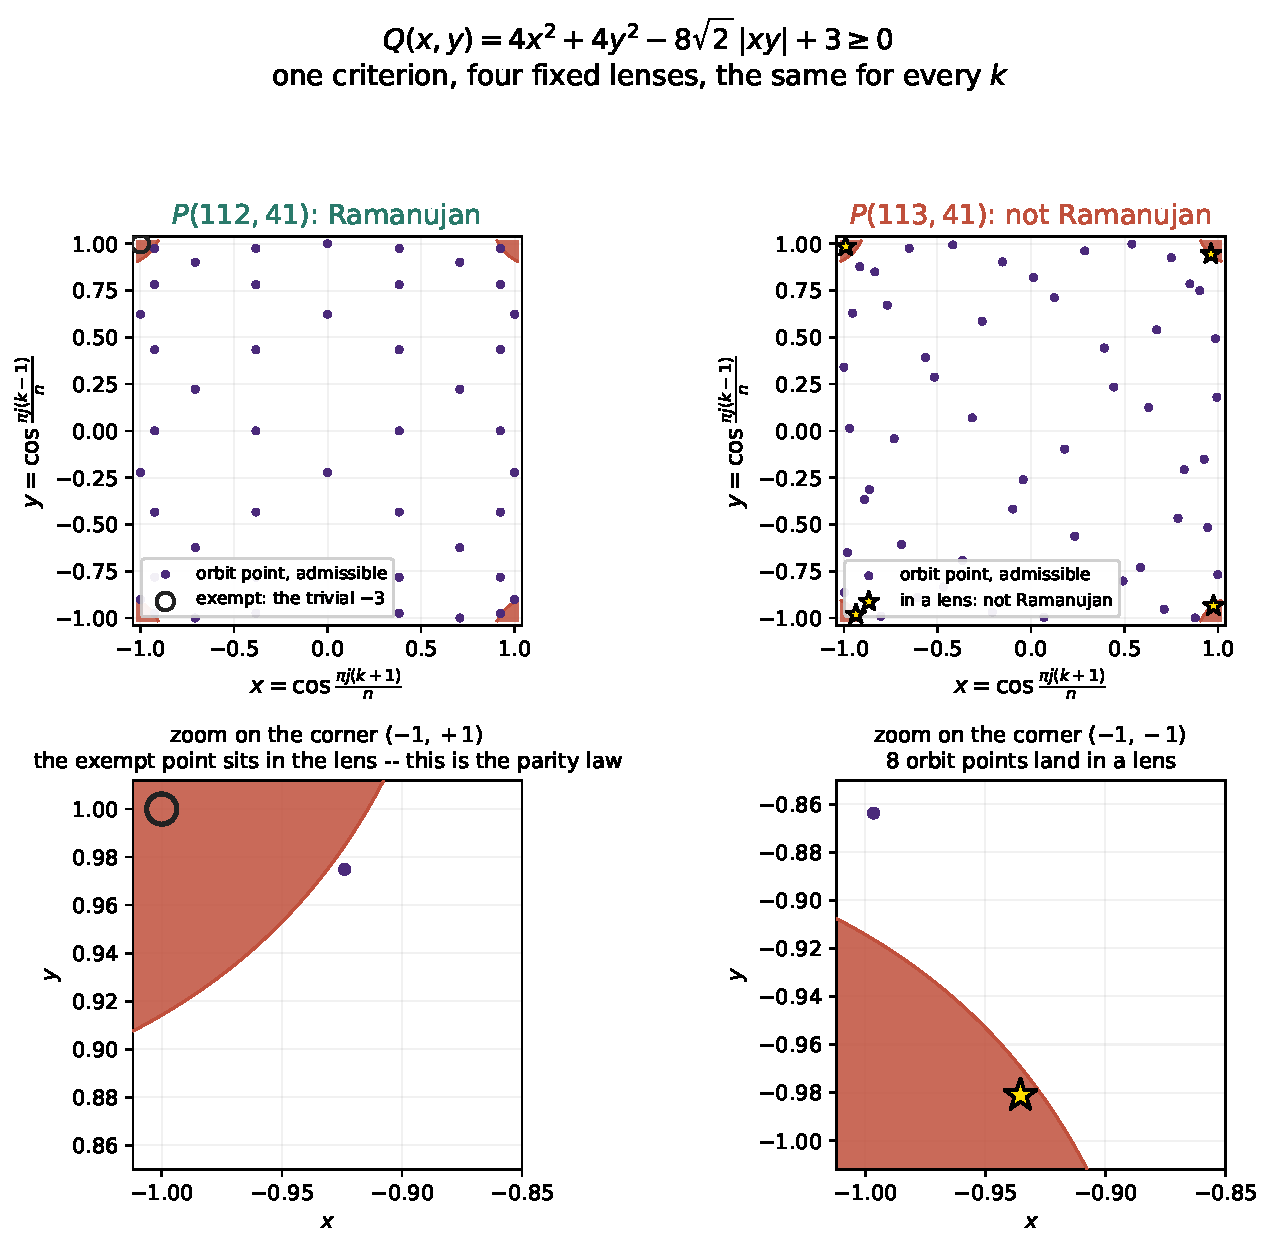
\includegraphics[width=\textwidth]{figures/fig_corner}
\caption{The corner criterion. Left, the largest Ramanujan member of the whole
family; right, the cover one step larger, which fails. The four forbidden
regions are the same in both pictures and for every $k$ --- only the map into
the square changes. In the left-hand zoom the single point inside a region is
the exempt trivial $-3$, which is why bipartiteness helps.}
\label{fig:corner}
\end{figure}

\section{Only finitely many, and a parity law}\label{sec:finite}

Both of the following come from the same observation: $D_k$ is negative at the
two points $u=\pm1$ where the grid $\{\cos(2\pi j/n)\}$ accumulates, so the grid
must \emph{clear} a band, and a fine grid cannot.

\begin{lemma}\label{lem:signs}
For every $k\ge1$,
\[
  D_k(1)=-7,\qquad D_k(0)\ge17,\qquad
  D_k(-1)=\begin{cases}-7,&k\text{ odd},\\ \ \ 9,&k\text{ even}.\end{cases}
\]
In particular $D_k$ has a root in $(0,1)$, and for odd $k$ also one in $(-1,0)$.
\end{lemma}

\begin{proof}
$T_k(1)=1$ gives $D_k(1)=11^2-8\cdot4^2=121-128=-7$. $T_k(-1)=(-1)^k$ gives
$D_k(-1)=(7-4(-1)^k)^2-8(2(-1)^k-2)^2$, which is $(-7)$ for $k$ odd and
$3^2-0=9$ for $k$ even. Finally $T_k(0)\in\{0,\pm1\}$, so
$D_k(0)=49-32\,T_k(0)^2\in\{49,17\}$. The sign changes give the roots.
\end{proof}

\begin{theorem}[Uniform finiteness, for every $k$]\label{thm:uniform}
Let $\tau=3-2\sqrt2=(\sqrt2-1)^2$. If $P(n,k)$ satisfies the Riemann Hypothesis
then
\[
  n\ \le\ \pi\bigl(2+\sqrt2\bigr)\sqrt{k^2+1},
\]
and if in addition $k$ and $n$ are both odd,
$n\le\tfrac12\pi(2+\sqrt2)\sqrt{k^2+1}$.
\end{theorem}

\begin{proof}
Write $x=\cos t$, $y=\cos kt$, and $a=1-x$, $b=1-y$, $s=a+b$. Suppose
$s<\tau$; then $a,b<\tau<1$, so $x,y>0$ and in particular $x+y>0$. Hence
$|A|=2(x+y)$ and $P=4xy$, and
\[
  G_k(t)=4\sqrt2\,(x+y)-4xy
        =\bigl(8\sqrt2-4\bigr)-\bigl(4\sqrt2-4\bigr)s-4ab .
\]
By AM--GM, $4ab\le s^2$, so $G_k(t)>7$ is implied by
\[
  s^2+\bigl(4\sqrt2-4\bigr)s\ <\ 8\sqrt2-11 .
\]
The left-hand side is increasing for $s\ge0$, and at $s=\tau$ it equals
\[
  (17-12\sqrt2)+(20\sqrt2-28)=8\sqrt2-11
\]
exactly. So $s<\tau$ suffices.

Now $1-\cos\theta\le\theta^2/2$ for every real $\theta$, whence
$s\le\bigl(1+k^2\bigr)t^2/2$, and therefore
\[
  0<t<\frac{\sqrt{2\tau}}{\sqrt{k^2+1}}=\frac{2-\sqrt2}{\sqrt{k^2+1}}
  \qquad\Longrightarrow\qquad G_k(t)>7,
\]
using $\sqrt{2\tau}=\sqrt{2}\,(\sqrt2-1)=2-\sqrt2$. The grid's smallest nonzero
angle is $2\pi/n$, so a Ramanujan $n$ needs
$2\pi/n\ge(2-\sqrt2)/\sqrt{k^2+1}$, i.e.\ $n\le2\pi\sqrt{k^2+1}/(2-\sqrt2)
=\pi(2+\sqrt2)\sqrt{k^2+1}$.

For the second bound take $k$ odd and put $t=\pi-\varphi$. Then $x=-\cos\varphi$
and, since $k$ is odd, $y=\cos(k\pi-k\varphi)=-\cos k\varphi$. With
$a'=1+x=1-\cos\varphi$ and $b'=1+y=1-\cos k\varphi$ and $s'=a'+b'<\tau$ we get
$x,y<0$, so $|A|=2(2-s')$ and $P=4(-1+a')(-1+b')$, and expanding gives
\emph{the same expression}
$\bigl(8\sqrt2-4\bigr)-\bigl(4\sqrt2-4\bigr)s'-4a'b'$. The rest of the argument
is verbatim, and $s'\le(1+k^2)\varphi^2/2$ as before. For odd $n$ the grid's
nearest point to $\pi$ is at $\varphi=\pi/n$, which gives the stated bound with
$\pi/n$ in place of $2\pi/n$ --- exactly half.
\end{proof}

\begin{remark}
An earlier draft of this work stated the same constant $\pi(2+\sqrt2)$, obtained
by expanding $\lambda_+$ to second order in $t$ at fixed $k$. That derivation is
\emph{invalid}: the critical $t$ scales like $1/k$, so $kt$ is of order one and
the expansion was used outside its domain. The constant survived numerical
testing only because the bound is loose. The proof above uses no expansion in
$kt$ at all --- only monotonicity, AM--GM, and $1-\cos\theta\le\theta^2/2$ ---
and holds for every $k$. The constant was right; the argument was not.
\end{remark}

\begin{theorem}[Finiteness]\label{thm:finite}
Let $u_k$ be the largest root of $D_k$ in $(-1,1)$. If $P(n,k)$ satisfies the
Riemann Hypothesis then
\[
  n\ \le\ \frac{2\pi}{\arccos u_k}\ =:\ B_k .
\]
In particular, for each $k$ only finitely many $n$ qualify.
\end{theorem}

\begin{proof}
By Lemma~\ref{lem:signs}, $D_k(1)=-7<0$, and $u_k$ is the largest root below
$1$, so $D_k<0$ throughout $(u_k,1]$. Suppose $n>B_k$. Then
$t=2\pi/n<\arccos u_k$, so $\cos t>u_k$ and hence $D_k(\cos t)<0$. The index
$j=1$ is never one of the two excluded indices of Corollary~\ref{cor:crit}
(that would need $n=2$), so Corollary~\ref{cor:crit} fails at $j=1$.
\end{proof}

Theorem~\ref{thm:uniform} is uniform but not sharp; for a \emph{given} $k$ the
exact root of $D_k$ does better, and that is what the classification uses.

Theorem~\ref{thm:uniform} bounds $n$ for each $k$, but the bound grows with
$k$, so it leaves open whether the family contains Ramanujan members of
arbitrarily large $k$. It does not, and the reason is that the failure
condition behind Theorem~\ref{thm:uniform} is a \emph{simultaneous Diophantine}
one, which Dirichlet's theorem satisfies unconditionally.

\begin{theorem}[Absolute finiteness]\label{thm:absolute}
If $n\ge231$ then $P(n,k)$ fails the Riemann Hypothesis for \emph{every} $k$.
Hence only finitely many generalized Petersen graphs satisfy it, and all of
them have $n\le230$.
\end{theorem}

\begin{proof}
The proof of Theorem~\ref{thm:uniform} shows that if
\[
  s=\bigl(1-\cos\tfrac{2\pi j}{n}\bigr)+\bigl(1-\cos\tfrac{2\pi jk}{n}\bigr)<\tau=3-2\sqrt2
\]
for even one nontrivial index $j$, then $P(n,k)$ is not Ramanujan. Writing
$\|\theta\|$ for the distance from $\theta$ to the nearest integer,
$1-\cos2\pi\theta=2\sin^{2}\pi\theta\le2\pi^{2}\|\theta\|^{2}$, so it is enough
that
\[
  \Bigl\|\tfrac jn\Bigr\|^{2}+\Bigl\|\tfrac{jk}{n}\Bigr\|^{2}
  \;<\;\frac{\tau}{2\pi^{2}}=0.0086919\ldots
\]
Let $J=\lfloor\sqrt n\rfloor$. Dirichlet's approximation theorem, applied to
the real number $k/n$, provides an integer $j$ with $1\le j\le J$ and
$\|jk/n\|\le1/(J+1)$. For that $j$ we have $J\le\sqrt n<J+1$, hence
\[
  \Bigl\|\tfrac jn\Bigr\|^{2}\le\Bigl(\tfrac Jn\Bigr)^{2}\le\frac1n,
  \qquad
  \Bigl\|\tfrac{jk}{n}\Bigr\|^{2}\le\frac{1}{(J+1)^{2}}<\frac1n ,
\]
so the left-hand side is less than $2/n$. Therefore $2/n<\tau/(2\pi^{2})$
suffices, that is
\[
  n\;>\;\frac{4\pi^{2}}{\tau}=230.097\ldots
\]
The index is legitimate: $1\le j\le\sqrt n<n/2$ once $n\ge5$, so $j$ is neither
$0$ nor the index $n/2$ that Corollary~\ref{cor:crit} excludes.
\end{proof}

\begin{remark}
The threshold $231$ is not sharp --- no Ramanujan $P(n,k)$ has $n$ above
$\RamAllMaxN$ --- and it does not need to be. Its only job is to be uniform in
$k$, which is exactly what the per-$k$ bound of Theorem~\ref{thm:finite} is
not. With it the classification becomes a finite problem in \emph{both}
variables: since $1\le k<n/2$, everything lives in $3\le n\le230$, a region
that can simply be exhausted.
\end{remark}

\begin{theorem}[Parity law]\label{thm:parity}
Let $k$ be odd and let $v_k$ be the smallest root of $D_k$ in $(-1,1)$. If $n$
is odd and $P(n,k)$ satisfies the Riemann Hypothesis then
\[
  n\ \le\ \frac{\pi}{\arccos(-v_k)} .
\]
No such restriction holds for even $n$, nor for even $k$.
\end{theorem}

\begin{proof}
For $k$ odd, $D_k(-1)=-7<0$ by Lemma~\ref{lem:signs}, so $D_k<0$ on
$[-1,v_k)$. The grid points nearest $t=\pi$ are $t=\pi(n\pm1)/n$ when $n$ is
odd, at distance $\pi/n$, with $\cos t=-\cos(\pi/n)$; and neither index is
excluded, since the excluded index $2j=n$ needs $n$ even. So the criterion
demands $-\cos(\pi/n)\ge v_k$, i.e.\ $\pi/n\ge\arccos(-v_k)$.

When $n$ is even the grid contains $t=\pi$ exactly, at $j=n/2$ -- and that is
precisely the index Corollary~\ref{cor:crit} excludes, because the sample there
is the trivial eigenvalue $-3$ of the bipartite graph. The band at $u=-1$ is
therefore invisible to even $n$. For even $k$, $D_k(-1)=9>0$ and there is no
band at $u=-1$ at all.
\end{proof}

The parity law is the reason the classification looks the way it does: for odd
$k$ the odd values of $n$ stop at roughly half the bound, and the tail of the
classification is even. It is also a small structural surprise -- \emph{being
bipartite helps}. Bipartiteness exempts the eigenvalue $-3$ from the Ramanujan
condition, and for odd $k$ that exemption is exactly what lets $n$ run twice as
far.

\section{The classification, certified exactly}\label{sec:ramcert}

Theorems~\ref{thm:finite} and~\ref{thm:parity} leave a finite computation, but a
finite computation is not yet a proof: the decision at a band edge is a
comparison of algebraic numbers, and that is where floating point fails
silently. We certify every case in exact arithmetic.

The mechanism is the one Corollary~\ref{cor:crit} makes available. Writing
$c_m=2\cos(2\pi jm/n)$ we have, by $4\cos a\cos b=2\cos(a+b)+2\cos(a-b)$,
\[
  A=c_1+c_k,\qquad P=c_{k+1}+c_{k-1},
\]
so $A$, $P$ and hence $D$ are values at $z=\zeta_n^{\,j}$ of Laurent
polynomials with integer coefficients. Since $\zeta_n^{\,j}$ is a primitive
$m$-th root of unity for $m=n/\gcd(n,j)$, each value is an algebraic integer of
$\mathbb Z[\zeta_m]$, and reducing modulo the cyclotomic polynomial $\Phi_m$
puts it in an exact integer coordinate vector. That vector vanishes if and only
if the value is exactly zero -- so the band-edge cases are decided by integer
arithmetic, with no estimate anywhere.

For the sign of a nonzero value we use the separation bound available to any
nonzero algebraic integer: the product of its conjugates is a nonzero rational
integer, so $|D|\ge1\big/\prod_{\sigma\ne1}|\sigma(D)|\ge 249^{-(\deg-1)}$,
using $|D|\le(7+4)^2+8\cdot4^2=249$ on the whole conjugate set. We evaluate at
a precision set from that bound and \emph{refuse} to report a sign unless the
computed value clears the guard, so a wrong sign is excluded rather than
improbable.

\begin{theorem}[Classification, per $k$]\label{thm:ramclass}
For every $k$ and every $n$, whether $P(n,k)$ satisfies the Riemann Hypothesis
is decided by Table~\ref{tab:ram}: for each $k$ listed there, the $n$ shown are
exactly those that qualify, and no $n>B_k$ qualifies, by
Theorem~\ref{thm:finite}. In particular there are exactly $\RamTotal$ such
graphs with $k\le\RamKmax$, from $\RamCases$ cases below the bound each decided
in exact arithmetic. That no $k$ beyond the table admits any $n$ at all is
Theorem~\ref{thm:absolute}, and the total is Theorem~\ref{thm:allk}.
\end{theorem}

\begin{table}[h]
\centering
\footnotesize
\setlength{\tabcolsep}{4pt}
% GENERATED by verification/verify_all.py -- do not edit by hand.
\begin{tabular}{r r r l}
\hline
$k$ & $B_k$ & count & the $n$ for which $P(n,k)$ satisfies the RH\\
\hline
$1$ & $15$ & $9$ & $3\text{--}8, 10, 12, 14$\\
$2$ & $23$ & $19$ & $5\text{--}23$\\
$3$ & $32$ & $18$ & $7\text{--}16, 18, 20, 22, 24, 26, 28, 30, 32$\\
$4$ & $42$ & $34$ & $9\text{--}42$\\
$5$ & $51$ & $28$ & $11\text{--}26, 28, 30, 32, 34, 36, 38, 40, 42, 44, 46, 48, 50$\\
$6$ & $61$ & $20$ & $13\text{--}16, 18, 20\text{--}23, 25, 27\text{--}28, 30, 32, 35, 37, 39, 42, 44, 49$\\
$7$ & $71$ & $39$ & $15\text{--}36, 38, 40, 42, 44, 46, 48, 50, 52, 54, 56, 58, 60, 62, 64, 66, 68, 70$\\
$8$ & $81$ & $16$ & $17, 19\text{--}22, 24, 26, 28\text{--}29, 31, 33, 35, 38, 40, 42, 49$\\
$9$ & $91$ & $50$ & $19\text{--}46, 48, 50, 52, 54, 56, 58, 60, 62, 64, 66, 68, 70, 72, 74, 76, 78, 80, 82, 84, 86, 88, 90$\\
$10$ & $101$ & $14$ & $21, 23, 25\text{--}26, 28, 30, 32, 34, 37, 39, 41, 43, 50, 52$\\
$11$ & $111$ & $36$ & $23\text{--}26, 28\text{--}32, 35\text{--}38, 40\text{--}42, 46\text{--}48, 50, 52\text{--}53, 58, 60, 62, 64, 70, 72, 74, 82, 84, 92, 94, 96, 104, 106$\\
$12$ & $121$ & $9$ & $27, 29\text{--}30, 32, 34, 38, 40, 45, 51$\\
$13$ & $131$ & $23$ & $28\text{--}30, 32, 34\text{--}37, 42\text{--}44, 46, 48\text{--}49, 56, 58, 60, 70, 72, 74, 84, 86, 98$\\
$14$ & $141$ & $7$ & $31, 33, 35\text{--}36, 38, 46, 53$\\
$15$ & $151$ & $19$ & $33\text{--}36, 38, 40\text{--}42, 49\text{--}50, 52, 54, 56, 66, 68, 70, 82, 84, 98$\\
$16$ & $161$ & $6$ & $35, 39\text{--}40, 42, 44, 52$\\
$17$ & $171$ & $16$ & $37\text{--}40, 42, 44, 46\text{--}47, 56, 58, 60, 62, 74, 76, 78, 94$\\
$18$ & $181$ & $3$ & $45\text{--}46, 50$\\
$19$ & $191$ & $17$ & $42\text{--}44, 46, 48, 50, 52\text{--}53, 64, 66, 68, 70, 84, 86, 88, 104, 106$\\
$20$ & $201$ & $3$ & $45, 49\text{--}50$\\
$21$ & $211$ & $11$ & $46, 48, 50, 54, 56, 58, 70, 72, 76, 92, 96$\\
$22$ & $221$ & $1$ & $49$\\
$23$ & $231$ & $10$ & $52\text{--}54, 56, 60, 62, 76, 78, 84, 106$\\
$24$ & $241$ & $1$ & $53$\\
$25$ & $251$ & $8$ & $56, 58, 60, 66, 68, 84, 90, 92$\\
$27$ & $271$ & $8$ & $60, 62, 64, 70, 72, 74, 90, 98$\\
$29$ & $291$ & $9$ & $64, 66, 68, 70, 76, 78, 96, 98, 106$\\
$31$ & $311$ & $4$ & $70, 74, 82, 84$\\
$33$ & $331$ & $5$ & $74, 76, 78, 86, 90$\\
$35$ & $351$ & $5$ & $78, 80, 84, 92, 96$\\
$37$ & $371$ & $3$ & $82, 84, 88$\\
$39$ & $391$ & $3$ & $88, 102, 106$\\
$41$ & $412$ & $2$ & $98, 112$\\
$43$ & $432$ & $2$ & $96, 98$\\
$45$ & $452$ & $2$ & $100, 108$\\
\hline
\multicolumn{4}{l}{\footnotesize No $k$ outside this table admits any $n$: the list is finite in both variables.}\\
\end{tabular}

\caption{The complete classification, every $n$ and every $k$. For each $k$,
$B_k$ is the per-$k$ bound of Theorem~\ref{thm:finite}; the rows stop at
$k=\RamAllMaxK$ because by Theorem~\ref{thm:absolute} no larger $k$ admits any
$n$ at all. Generated directly from the certification run.}
\label{tab:ram}
\end{table}

The bound is not merely finite but frequently sharp: at $k=2,3,4$ the largest
Ramanujan $n$ equals $\lfloor B_k\rfloor$ exactly, so the band at $u=1$ is the
only obstruction there, and the parity bound of Theorem~\ref{thm:parity} is
attained at $k=1,5,7,9$.

A floating-point classifier was run alongside the exact one throughout, as a
control with no authority: a disagreement is recorded as a failure of the run
rather than resolved in favour of either. It earned its place. At $k=1$ the
exponents of the Laurent polynomials collide ($k=1$ and $k-1=-(k-1)=0$), and an
implementation that built them as a dictionary literal silently discarded the
duplicated terms; the exact classifier then declared every $P(n,1)$ Ramanujan,
including $P(9,1)$, whose spectrum contains $2\cos(8\pi/9)-1=-2.879$. The
control caught all four affected values.

\begin{remark}
The classification is genuinely irregular in $k$. The largest Ramanujan $n$ is
not monotone --- $k=9$ reaches $n=\RamLastNine$ while $k=8$ and $k=10$ stop at
$\RamLastEight$ and $\RamLastTen$ --- because for even $k$ a third band, interior
to $(0,\pi)$ rather than at an endpoint, binds well before the band at $u=1$.
Locating those interior bands for general $k$ is exactly the question of which
cyclotomic reals avoid a semialgebraic set, and is where the Galois-orbit
machinery of Part~\ref{part:zf} applies.
\end{remark}

\section{The classification for every \texorpdfstring{$k$}{k}}\label{sec:allk}

Theorem~\ref{thm:absolute} confines the whole family to $3\le n\le230$, and
with $1\le k<n/2$ that region is finite. Exhausting it settles the question
completely.

\begin{theorem}[Complete classification]\label{thm:allk}
There are exactly $\RamAllTotal$ pairs $(n,k)$ with $n\ge3$ and $1\le k<n/2$
for which $P(n,k)$ satisfies the Riemann Hypothesis. They fall into
$\RamAllIso$ isomorphism classes. The largest is $n=\RamAllMaxN$, attained at
$k=41$; the largest $k$ that occurs at all is $\RamAllMaxK$; and the values of
$k$ that occur are $1,\dots,25$ together with the odd numbers from $27$ to
$\RamAllMaxK$. Every one of the $\RamAllCases$ cases in the region was decided
in exact arithmetic.
\end{theorem}

Two features of the answer are worth isolating. The first is that the list is
finite in \emph{both} variables, which Theorem~\ref{thm:uniform} alone does not
give: for each $k$ it allows $n$ up to $\pi(2+\sqrt2)\sqrt{k^{2}+1}$, a bound
that grows without limit, and only the Diophantine argument rules out large
$k$. The second is the parity asymmetry at the top of the range. Above $k=25$
no even $k$ occurs at all, while odd $k$ persists as far as $\RamAllMaxK$; this
is the parity law of Theorem~\ref{thm:parity} still operating at the end of the
list, where the exemption of the trivial $-3$ is the only thing keeping a
member alive.

\begin{remark}[Counting graphs rather than parameters]
$\RamAllTotal$ counts parameter pairs. $P(n,k)\cong P(n,\ell)$ exactly when
$\ell\equiv\pm k^{\pm1}\pmod n$, and quotienting by that relation leaves
$\RamAllIso$ graphs up to isomorphism. We report both because the first is
what the criterion decides and the second is what the classification is
\emph{about}; conflating them would overstate the count by a third.
\end{remark}

\section{Towards a closed form}\label{sec:closed}

Theorem~\ref{thm:allk} is a certified list, not a formula, and it is worth
being precise about what a formula would have to be. This section gives the
structure the list has; it stops short of a closed form, and \S\ref{sec:closed}
ends by saying exactly where.

The first observation is that the criterion is \emph{local at the divisors of
$n$}. Call $m$ the \emph{level} of the index $j$ if $m=n/\gcd(n,j)$; then
$\cos\frac{2\pi j}{n}$ is a primitive $m$-th value, and as $j$ ranges over all
indices of level $m$ the point ranges over the full conjugate set
$\{\cos\frac{2\pi i}{m}:\gcd(i,m)=1\}$. Say $m$ is \emph{bad for $k$} if some
primitive level-$m$ point violates $Q\ge0$.

\begin{theorem}[Locality]\label{thm:local}
$P(n,k)$ satisfies the Riemann Hypothesis if and only if no divisor $m\ge3$ of
$n$ is bad for $k$. Moreover badness at level $m$ depends on $k$ only through
$k\bmod m$.
\end{theorem}

\begin{proof}
Every index $j\in\{1,\dots,n-1\}$ has a level $m\mid n$, and $m\ge3$ unless
$j=0$ or $2j=n$ --- the two indices Corollary~\ref{cor:crit} excludes. Level
$m=2$ never obstructs in any case: there $u=-1$, and $D_k(-1)=9>0$ for even $k$
by Lemma~\ref{lem:signs}, while for odd $k$ the cover is bipartite and the point
carries the exempt trivial $-3$. So the criterion holds at every index exactly
when it holds at every primitive point of every level $m\ge3$ dividing $n$. The
last claim holds because the point
$\bigl(\cos\frac{\pi j(k+1)}{m},\cos\frac{\pi j(k-1)}{m}\bigr)$ is unchanged
when $k$ is replaced by $k+m$.
\end{proof}

\begin{corollary}[Divisor closure]\label{cor:divclosed}
If $P(n,k)$ satisfies the Riemann Hypothesis and $d\mid n$ with $d>2k$, then
$P(d,k)$ does too. For each $k$ the set of Ramanujan $n$ is closed downwards
under division, so it is determined by its minimal bad divisors --- and by
Theorem~\ref{thm:finite} only those below $B_k$ can matter.
\end{corollary}

\begin{proof}
The divisors of $d$ are divisors of $n$, so if none of the latter is bad for $k$
then none of the former is; apply Theorem~\ref{thm:local} twice.
\end{proof}

That reduces the classification to knowing which $(m,k\bmod m)$ are bad. The
next lemma is what converts that into arithmetic, and it is where the $\gcd$
enters.

\begin{lemma}[The minimum is a gcd]\label{lem:mingcd}
Let $\|\cdot\|$ denote distance to the nearest integer. If $m\nmid c$ then
\[
  \min\Bigl\{\,\Bigl\|\tfrac{jc}{m}\Bigr\|\ :\ \gcd(j,m)=1\,\Bigr\}
  \ =\ \frac{\gcd(c,m)}{m}.
\]
If $m\mid c$ the minimum is $0$.
\end{lemma}

\begin{proof}
Write $g=\gcd(c,m)$, $c=ga$, $m=gb$ with $\gcd(a,b)=1$, and $b>1$ since
$m\nmid c$. Then $jc\equiv g\,(ja)\pmod m$, so $\|jc/m\|=\|ja/b\|$ scaled: the
attainable residues are $g\,t$ with $t\equiv ja\pmod b$. As $j$ runs over the
units mod $m$, $j\bmod b$ runs over the units mod $b$, and $a$ is a unit there,
so $ja\bmod b$ runs over every unit of $b$ --- in particular over $1$. The
smallest nonzero residue attainable is therefore $g$, giving $g/m$, and $0$ is
not attainable because $b\nmid ja$ for $j$ a unit.
\end{proof}

Now the geometry pays. Corollary~\ref{cor:lens} showed the forbidden region
meets the sides of the square at distance $\tfrac32-\sqrt2$ from each corner, so
$Q<0$ forces \emph{both} $|x|$ and $|y|$ to be at least $\sqrt2-\tfrac12$. Since
$|\cos\pi t|\ge\sqrt2-\tfrac12$ exactly when $\|t\|\le\gamma$ for
\[
  \gamma=\frac{\arccos\bigl(\sqrt2-\tfrac12\bigr)}{\pi}=0.1328095\ldots,
  \qquad \frac1\gamma=7.5295\ldots,
\]
a level is safe as soon as one coordinate cannot come close enough --- and by
Lemma~\ref{lem:mingcd} that is a divisibility condition. Because $m/\gcd(k\pm1,m)$
is an integer and $1/\gamma$ is just above $7$, it is a condition on small
integers.

\begin{theorem}[Gcd safety]\label{thm:gcdsafe}
If $m/\gcd(k+1,m)\in\{2,\dots,7\}$ or $m/\gcd(k-1,m)\in\{2,\dots,7\}$, then $m$
is not bad for $k$.
\end{theorem}

\begin{proof}
Suppose $m/\gcd(k+1,m)=b$ with $2\le b\le7$. Then $m\nmid k+1$, so
Lemma~\ref{lem:mingcd} gives $\|j(k+1)/m\|\ge\gcd(k+1,m)/m=1/b\ge1/7>\gamma$ for
every $j$ coprime to $m$. Hence $|x|=|\cos\frac{\pi j(k+1)}{m}|<\sqrt2-\tfrac12$
at every primitive level-$m$ point, and $Q\ge0$ there by
Corollary~\ref{cor:lens}. The other case is identical.
\end{proof}

The value $b=1$ is excluded for a reason: $m\mid k+1$ pins $|x|=1$, which is the
worst case rather than the best, and Lemma~\ref{lem:mingcd} gives minimum $0$.

Theorem~\ref{thm:local} already gives the classification a pure form for
\emph{every} $k$: $P(n,k)$ is Ramanujan iff no divisor $m\ge3$ of $n$ is bad
for $k\bmod m$, and badness of a level is witnessed by a single index $j$ with
$Q<0$, an exact one-line check. Since $m\le\RamDirichlet$ by
Theorem~\ref{thm:absolute}, the whole classification is one theorem plus a
finite table of minimal bad levels (a few thousand pairs $(m,k\bmod m)$,
generated and stored with the verification record); the list of
$\RamAllTotal$ pairs is a consequence of that table, not the primary object.
For small $k$ the two bounds already in hand turn out to be the whole answer,
and this can be \emph{proved}, not merely checked: everything depends on where
$D_k$ is negative, and that is a question about the real roots of one integer
polynomial, which Sturm's theorem decides in integer arithmetic.

\begin{lemma}[Band structure]\label{lem:bands}
Let $u_k$ be the largest root of $D_k$ in $(-1,1)$. For
$k\in\{1,2,3,4,5,7,9\}$ the set where $D_k<0$ on $[-1,1]$ is exactly
\[
  (u_k,1]\quad(k\ \text{even}),\qquad\qquad [-1,-u_k)\cup(u_k,1]\quad(k\ \text{odd}).
\]
For $k=6,8$ and for every $k$ with $10\le k\le45$, $D_k$ has a further root in
$(-1,1)$ and is negative on an interval in the interior.
\end{lemma}

\begin{proof}
For odd $k$ the Chebyshev polynomial $T_k$ is odd, so $uT_k(u)$ is even and
$(2u+2T_k(u))^2$ is even; hence $D_k(-u)=D_k(u)$ and the roots come in pairs
$\pm u$, with $v_k=-u_k$ in the notation of Theorem~\ref{thm:parity}. For even
$k$, $D_k(-1)=9>0$ by Lemma~\ref{lem:signs}, so there is no band at $-1$. The
number of real roots of $D_k$ in $[-1,1]$, and the sign of $D_k$ between
consecutive roots, are decided by Sturm's theorem, a finite computation in
integer arithmetic on the coefficients of $D_k\in\mathbb Z[u]$; carried out
exactly for $k\le45$ (\texttt{verification/interior\_bands.py}, which isolates
the roots over $\mathbb Q$ and evaluates $D_k$ at rational points between them),
it finds one root in $(-1,1)$ for $k=2,4$, two for $k=1,3,5,7,9$, and at least
three for every other $k\le45$, with the signs stated. For $k=2$ the whole
computation fits on a page: $D_2(u)=64u^6-192u^4-16u^3+112u^2+8u+17$ has
$D_2(-1)=9$, $D_2(0.96)=0.765\ldots>0$ and $D_2(1)=-7$; Sturm's theorem gives
$D_2$ no root in $[-1,0.96]$, and $D_2'$ no root in $(0.96,1)$, so $D_2$ is
positive on $[-1,0.96]$ and crosses zero exactly once in $(0.96,1)$, at
$u_2=0.9641\ldots$.
\end{proof}

\begin{theorem}[Closed form for $k\le9$]\label{prop:closedsmall}
Let $B_k=2\pi/\arccos u_k$ be the bound of Theorem~\ref{thm:finite} and
$P_k=\pi/\arccos u_k=B_k/2$ that of Theorem~\ref{thm:parity}. Then
\[
\begin{array}{ll}
  k=2,4: & P(n,k)\ \text{is Ramanujan}\iff 2k<n\le B_k;\\[2pt]
  k=1,3,5,7,9: & P(n,k)\ \text{is Ramanujan}\iff 2k<n\le B_k\ \text{and }
  (n\ \text{even or}\ n\le P_k).
\end{array}
\]
Equivalently, for odd $k$: $2k<n\le B_k$ and every odd divisor of $n$ is at most
$P_k$.
\end{theorem}

\begin{proof}
By Theorem~\ref{thm:crit}, $P(n,k)$ is Ramanujan iff $D_k(\cos\frac{2\pi j}{n})\ge0$
for every $j$ with $1\le j\le n-1$ and $j\ne n/2$. By Lemma~\ref{lem:bands},
$D_k(\cos t)<0$ exactly when $\cos t>u_k$, or $k$ is odd and $\cos t<-u_k$.

\emph{The band at $1$.} Among $1\le j\le n-1$ the largest value of
$\cos\frac{2\pi j}{n}$ is $\cos\frac{2\pi}{n}$, at $j=1$ and $j=n-1$. So some
grid point lies in $(u_k,1]$ iff $\cos\frac{2\pi}{n}>u_k$ iff $n>B_k$.

\emph{The band at $-1$ (odd $k$).} Write $d=n-2j$, so that
$\cos\frac{2\pi j}{n}=-\cos\frac{\pi d}{n}$, and $d\ne0$ because $j=n/2$ is the
excluded trivial index. A grid point lies in $[-1,-u_k)$ iff
$\cos\frac{\pi d}{n}>u_k$ for some admissible $d$, and the admissible $|d|$ are
the positive integers of the same parity as $n$. The smallest is $2$ when $n$ is
even, giving the condition $\cos\frac{2\pi}{n}>u_k$ again, i.e.\ $n>B_k$; and
$1$ when $n$ is odd, giving $\cos\frac{\pi}{n}>u_k$, i.e.\ $n>P_k$.

The lower bound $2k<n$ is the standing hypothesis $k<n/2$. For the equivalent
form: an even $n\le B_k$ has every odd divisor at most $n/2\le P_k$, and an odd
$n$ is its own odd divisor.
\end{proof}

For even $k$ there is no band at $u=-1$ at all, which is why $k=2$ and $k=4$
are unbroken runs; for odd $k$ the second band contributes exactly the
constraint that $n$ carry no large odd divisor, which by
Corollary~\ref{cor:divclosed} is the natural form for a divisor-closed set to
take. The thresholds themselves --- $\lfloor B_k\rfloor$ and $\lfloor P_k\rfloor$
--- are $\lfloor B_k\rfloor=\RamLastTwo,\RamLastThree,\RamLastFour,\RamLastFive,\RamLastSeven,\RamLastNine$
at $k=2,3,4,5,7,9$ (Table~\ref{tab:ram}); deciding whether
$\cos\frac{2\pi}{n}\le u_k$ at the boundary $n$ is one exact comparison in
$\mathbb Z[\zeta_n]$, as in \S\ref{sec:ramcert}.

\begin{remark}[What a closed form still needs, and why we do not have one]
Three things are missing. Theorem~\ref{thm:gcdsafe} is \emph{sufficient and
one-sided}: it certifies safety and says nothing about badness, and a closed
form needs both directions. Theorem~\ref{prop:closedsmall} stops at
$k=6,8$ and at every $k\ge10$ --- precisely where Lemma~\ref{lem:bands} finds an
interior band, neither at $u=1$ nor at $u=-1$, and locating which grid points
fall into those bands is the question of which cyclotomic reals avoid a
semialgebraic set that \S\ref{sec:ramcert} already flagged. And nothing here explains the shape of the
answer at the top of the range: we can prove no $P(n,k)$ with
$k>\RamAllMaxK$ is Ramanujan, but only by exhausting the finitely many cases
Theorem~\ref{thm:absolute} leaves, and we cannot say why the cut falls at
$\RamAllMaxK$ rather than near it. The list is complete and certified; it is
not yet explained.
\end{remark}

\section{Every cubic cyclic cover}\label{sec:covram}

Nothing in \S\ref{sec:corner} used $P(n,k)$ beyond two facts: the base has two
vertices, and the cover is cubic. The criterion therefore belongs to the
setting of \S\ref{sec:covers} rather than to this family, and saying so turns
a classification of one family into a statement about a class of covers.

A cubic base on two vertices is one of exactly two things. A loop absorbs two
of the three half-edges at its vertex, so a vertex carries at most one loop,
and a vertex with a loop has exactly one non-loop edge. Either both vertices
carry loops --- the \emph{two-loop base} $B(a,b,c)$, with a loop of voltage $a$
at $u$, a loop of voltage $b$ at $v$, and an edge $u\!-\!v$ of voltage $c$ ---
or neither does, leaving three parallel edges, the \emph{theta base}
$T(c_1,c_2,c_3)$. We have $P(n,k)=B(1,k,0)^{n}$, and the covers of a theta base
are the cubic cyclic Haar graphs, which are bipartite.

\begin{theorem}[Corner criterion on a two-loop base]\label{thm:covcorner}
Let $X=B(a,b,c)^{n}$ be simple and connected. Then $X$ satisfies the Riemann
Hypothesis if and only if
\[
  Q\Bigl(\cos\tfrac{\pi j(a+b)}{n},\ \cos\tfrac{\pi j(a-b)}{n}\Bigr)\ \ge\ 0
\]
at every nontrivial index, with $Q$ the form of Theorem~\ref{thm:corner}.
In particular the spectrum, and hence the answer, does not depend on the edge
voltage $c$ at all.
\end{theorem}

\begin{proof}
By Theorem~\ref{thm:cover} the character block is
$M_j=\begin{psmallmatrix}\alpha_j&\omega^{jc}\\ \omega^{-jc}&\beta_j\end{psmallmatrix}$
with $\alpha_j=2\cos\frac{2\pi ja}{n}$ and $\beta_j=2\cos\frac{2\pi jb}{n}$.
Its characteristic polynomial is $\lambda^{2}-(\alpha+\beta)\lambda+(\alpha\beta-|\omega^{jc}|^{2})$,
and $|\omega^{jc}|=1$, so it is $\lambda^{2}-A\lambda+(P-1)$ exactly as in
Lemma~\ref{lem:blocks} --- with no $c$ in it. The derivation of
Theorem~\ref{thm:crit} used only $|\alpha|,|\beta|\le2$, so it applies verbatim,
and the substitution of Theorem~\ref{thm:corner} applies with $a+b$ and $a-b$
in place of $k+1$ and $k-1$, because
$\alpha+\beta=4\cos\frac{\pi j(a+b)}{n}\cos\frac{\pi j(a-b)}{n}$ and
$\alpha\beta=2\bigl(\cos\frac{2\pi j(a+b)}{n}+\cos\frac{2\pi j(a-b)}{n}\bigr)$.
\end{proof}

\begin{theorem}[Theta base]\label{thm:thetarh}
$T(c_1,c_2,c_3)^{n}$ satisfies the Riemann Hypothesis if and only if
\[
  \sum_{l<m}\cos\frac{2\pi j(c_l-c_m)}{n}\ \le\ \frac52
  \qquad\text{for every }j\ne0 .
\]
\end{theorem}

\begin{proof}
The block is $\begin{psmallmatrix}0&S_j\\ \overline{S_j}&0\end{psmallmatrix}$
with $S_j=\sum_l\omega^{jc_l}$, so its eigenvalues are $\pm|S_j|$ and the cover
is bipartite. Now $|S_j|^{2}=3+2\sum_{l<m}\cos\frac{2\pi j(c_l-c_m)}{n}$, and
the Ramanujan condition on a nontrivial index is $|S_j|^{2}\le8$.
\end{proof}

\begin{theorem}[Uniform finiteness on both bases]\label{thm:covfinite}
Writing voltages by their representatives of least absolute value, and $d_1,d_2,d_3$
for the pairwise differences $c_l-c_m$,
\begin{align*}
  B(a,b,c)^{n}\ \text{Ramanujan}\ &\Longrightarrow\ n\le\pi(2+\sqrt2)\sqrt{a^{2}+b^{2}},\\
  T(c_1,c_2,c_3)^{n}\ \text{Ramanujan}\ &\Longrightarrow\ n\le2\pi\sqrt{d_1^{2}+d_2^{2}+d_3^{2}} .
\end{align*}
\end{theorem}

\begin{proof}
The first is the proof of Theorem~\ref{thm:uniform} with $\cos\frac{2\pi ja}{n}$
and $\cos\frac{2\pi jb}{n}$ in place of $\cos t$ and $\cos kt$; the estimate
$1-\cos\theta\le\theta^{2}/2$ now gives $s\le(a^{2}+b^{2})\theta^{2}/2$, and
setting $\theta=2\pi/n$ gives the bound. Specialising to $(a,b)=(1,k)$ returns
Theorem~\ref{thm:uniform} exactly. For the second, the condition of
Theorem~\ref{thm:thetarh} fails as soon as $\sum_l(1-\cos\frac{2\pi jd_l}{n})<\tfrac12$,
and that sum is at most $\theta^{2}\sum_ld_l^{2}/2$; at $j=1$ this forces
failure once $2\pi/n<1/\sqrt{\sum d_l^{2}}$.
\end{proof}

The second bound is sometimes attained exactly: for $T(0,1,2)$ it reads
$n\le2\pi\sqrt6=15.39\ldots$, and $n=15$ is Ramanujan.

Both bases are therefore finite, and the reason is not special to two-vertex
bases.

\begin{theorem}[No infinite family is a cyclic cover]\label{thm:noinfinite}
Let $B$ be a fixed finite connected cubic base with integer voltages. Then
$B^{n}$ is Ramanujan for only finitely many $n$. Explicitly, writing $L$ for
$\sqrt2\sum|v_e|$ over the non-loop edges and $R$ for $\sum v_e^{2}$ over the
loops, $B^{n}$ is not Ramanujan as soon as
\[
  \frac{2\pi}{n}L+\Bigl(\frac{2\pi}{n}\Bigr)^{2}R\;<\;\tau=3-2\sqrt2 .
\]
\end{theorem}

\begin{proof}
$M_0$ is the adjacency matrix of the base, which is $3$-regular, so its largest
eigenvalue is $3$. A non-loop edge of voltage $v$ moves two entries of $M_1$ by
$|\omega^{v}-1|\le2\pi|v|/n$ each, and a loop of voltage $v$ moves one entry by
$|2\cos\frac{2\pi v}{n}-2|\le(2\pi v/n)^{2}$; summing gives
$\|M_1-M_0\|_2\le\|M_1-M_0\|_F\le\frac{2\pi}{n}L+(\frac{2\pi}{n})^{2}R$. By
Weyl's inequality $\lambda_{\max}(M_1)\ge3-\|M_1-M_0\|_2$, and $\lambda_{\max}(M_1)$
is a nontrivial eigenvalue, since in a connected cover the eigenvalue $3$ has
multiplicity one and occurs at $j=0$. So once the displayed quantity is below
$3-2\sqrt2$ the cover has a nontrivial eigenvalue exceeding $2\sqrt2$.
\end{proof}

\begin{remark}[What this is, and is not]
Theorem~\ref{thm:noinfinite} says that no construction of the kind this paper
studies can produce an infinite family of Ramanujan graphs --- the no-go is a
property of the class, not a limitation of our search. We claim no novelty for
the principle: it is the cyclic instance of the familiar fact that abelian
covers do not expand, which is precisely why the Lubotzky--Phillips--Sarnak
construction \cite{lps} is built on $\mathrm{PGL}_2$ and not on a cyclic group.
What is new here is the explicit constant, and the two exact criteria of
Theorems~\ref{thm:covcorner} and~\ref{thm:thetarh} for the two-vertex bases,
which decide the finitely many surviving cases rather than merely bounding
them.
\end{remark}

\section{The deficit: what the no-go costs}\label{sec:deficit}

A classification that ends in a finite list tells a designer that beyond a
certain size there is nothing optimal to build. That is not by itself useful
advice. The useful quantity is how much is lost, and the criterion supplies it
in closed form.

\begin{definition}
For a cover with nontrivial spectral radius $\lambda_2$, the \emph{deficit} is
$\delta=\lambda_2-2\sqrt2$, and for a given size,
$\delta^{*}(n)=\min_{1\le k<n/2}\delta(n,k)$.
\end{definition}

$\delta^{*}(n)\le0$ exactly when some $P(n,k)$ is Ramanujan, which by
Theorem~\ref{thm:allk} happens for exactly $\RamAllSizes$ values of $n$, the
largest being $\RamAllMaxN$.

\begin{proposition}\label{prop:deficit}
$\delta(n,k)<3-2\sqrt2$ for every $n$ and $k$, and
$\sup_{n,k}\delta(n,k)=3-2\sqrt2$, approached as $n\to\infty$.
\end{proposition}

\begin{proof}
$\lambda_2<3$ because $3$ is simple in a connected cubic graph, which gives the
bound. For the supremum, at $j=1$ the block $M_1$ tends to $M_0$ as
$n\to\infty$, so its top eigenvalue tends to $3$, and it is nontrivial.
\end{proof}

So the loss is bounded, and the bound is exactly the gap $\tau$ that the whole
argument has been about: an engineer who builds at a size where no optimal
member exists gives up at most $3-2\sqrt2=0.1716\ldots$ in nontrivial spectral
radius, and that is the worst case rather than a typical one.
Figure~\ref{fig:deficit} plots $\delta^{*}$. Its two branches are the parity
law once more: for one parity of $n$ the exemption of the trivial $-3$ is
available and for the other it is not.

\begin{figure}[h]
\centering
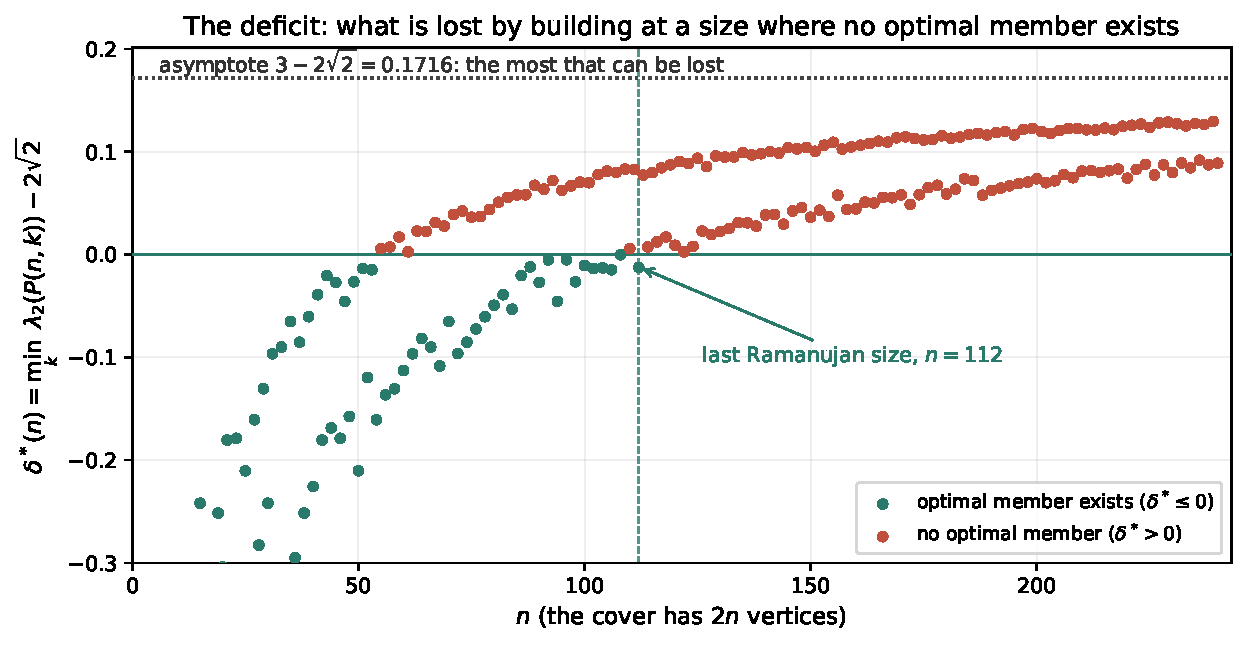
\includegraphics[width=\textwidth]{figures/fig_deficit}
\caption{The deficit $\delta^{*}(n)$, the best achievable nontrivial spectral
radius at each size, measured from the Ramanujan threshold. Green points are
sizes at which an optimal member exists; the last is $n=\RamAllMaxN$. The
curve rises to the asymptote $3-2\sqrt2$, which by
Proposition~\ref{prop:deficit} is the most that can ever be lost. The two
branches are the parity law.}
\label{fig:deficit}
\end{figure}
